В настоящее время значения основных космологических параметров известны с очень высокой точностью. В рамках современной стандартной космологической модели $\Lambda$CDM некоторые из них определены с точностью один процент или лучше (\cite{planck2018}). Однако для некоторых параметров, например, для постоянной Хаббла $H_0$, определяющей  темп расширения Вселенной в современную эпоху, наблюдается систематическое расхождение в значениях,  измеренных по ранней и по поздней Вселенной (см. Рис. \ref{fig:h0s}). Например, по данным обcерватории \textit{Planck} из наблюдений реликтового излучения величина $H_0$ составляет $67.4 \pm 0.5$ км/с/Мпк (\cite{planck2018}); в то же время из наблюдений сверхновых типа Ia, так называемых «стандартных свечей», получено не зависящее от используемой космологической модели значение постоянной Хаббла, равное $74.03 \pm 1.42$ км/с/Мпк (\cite{riess2019}).  Эти значения не согласуются друг с другом на уровне значимости примерно $4.4\sigma$, что может свидетельствовать как о наличии неучтенных или неизвестных систематических эффектов, так и о новой физике, выходящей за рамки модели $\Lambda$CDM. Для понимания причин этого расхождения необходимо привлечение независимых подходов, способных также с высокой точностью определять фундаментальные космологические параметры, одним из которых является использование наблюдений гравитационно линзированных систем.

\begin{figure}[h]
    \centering
	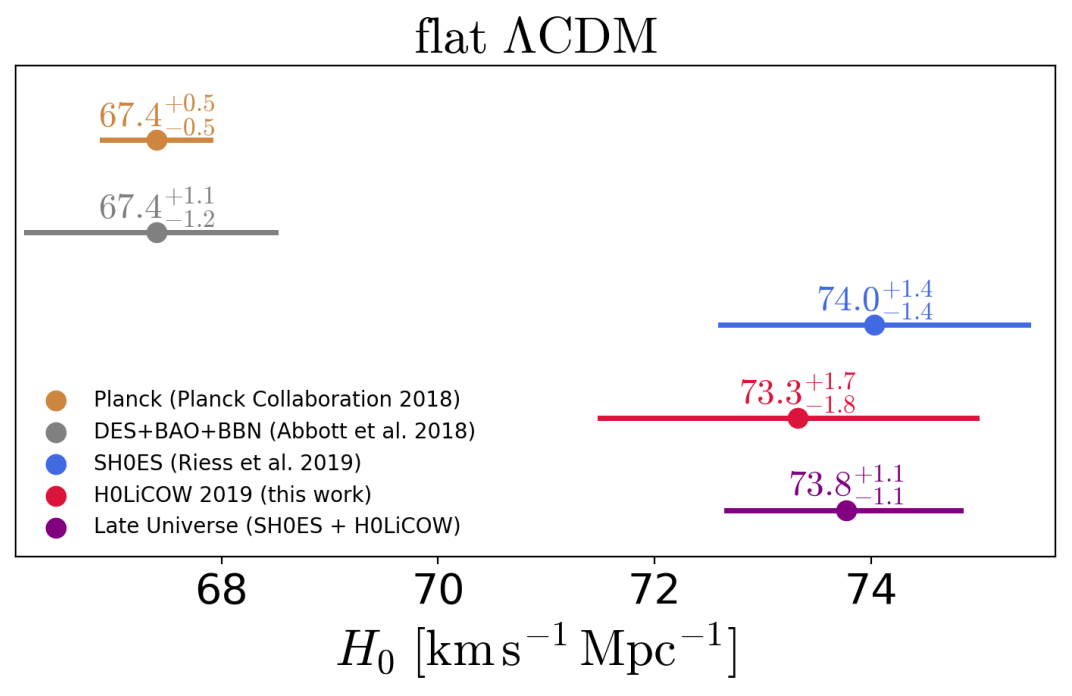
\includegraphics[width=0.80\textwidth]{pics/h0s.png}
	\caption{Сравнение значений $H_0$ (\cite{holicowXIII}) в предположении плоской модели $\Lambda$CDM. Измерения по ранней Вселенной представлены обзором обсерватории \textit{Planck} (оранжевый, \cite{planck2018}) и комбинацией наблюдений Dark Energy Survey, барионно-аккустических осцилляций и первичного нуклеосинтеза (серый, \cite{abbott2018b}). Измерения по поздней Вселенной представлены результатами работы коллабораций SH0ES (синий, \cite{riess2019}) и H0LICOW (красный, \cite{holicowXIII}), а также их комбинацией (фиолетовый), для которой наблюдается расхождение на уровне $5.3\sigma$ с данными \textit{Planck}.}
	\label{fig:h0s}
\end{figure} 

Гравитационное линзирование -- это отклонение  траектории света от прямолинейной в гравитационном поле массивных объектов (см., например, классические учебники по теории гравитационного линзирования: \cite{schneider1992}, \cite{gravlensbook}). Важным свойством гравитационного линзирования является возможность формирования нескольких изображений одного и того же источника. Если линзированный источник является переменным, то точное измерение временной задержки между кривыми блеска, наблюдаемыми в различных изображениях, позволяет с высокой точностью оценить значение постоянной Хаббла (\cite{timedelaycosmography}), а также других космологических параметров (\cite{holicowXIII}).

В настоящее время в целях уточнения космологических параметров активно развиваются методы, основанные на анализе наблюдаемых гравитационно линзированных квазаров. Многолетние наблюдения множественных изображений линзированных галактиками квазаров позволили с хорошей точностью измерить временные запаздывания между их изображениями. В рамках проекта COSMOGRAIL (\textit{COSmological MOnitoring of GRAvitational Lenses}) уже более десяти лет проводятся регулярные наблюдения кривых блеска примерно тридцати линзированных квазаров и разрабатываются методы определения временных запаздываний с целью определения постоянной Хаббла с точностью $\sim$3\%, что уже сравнимо с точностью, полученной из наблюдений обсерватории \textit{Planck} (\cite{cosmograil}). Однако в ходе выполнения данного проекта выяснилось, что проблема вырождения между гравитационным потенциалом линзы и постоянной Хаббла не позволяет достичь заявленной точности без привлечения дополнительной информации. В связи с этим был инициирован новый проект H0LiCOW (\textit{$H_0$ Lenses in COSMOGRAIL's Wellspring}), в рамках которого для анализа были выбраны пять гравитационно-линзированных квазаров, для которых проводятся дополнительные фотометрические и спектроскопические наблюдения с высоким разрешением, в том числе измерения дисперсии скоростей звезд в галактике-линзе. Это позволит получить распределение массы в линзирующей галактике с точностью до нескольких процентов и оценить постоянную Хаббла с точностью <3.5\% (\cite{holicowI}). Важно отметить, что надежные измерения временных запаздываний между изображениями квазаров из наблюдений их кривых блеска требуют длительного (более 10 лет) мониторинга. Это связано с наличием как микролинзирования, так и возможной внутренней переменности квазаров на схожих с микролинзированием масштабах.

В последние годы также развивается направление исследования сверхновых, которые линзированы галактиками или скоплениями галактик. Идея использования линзированных сверхновых для оценки $H_0$ была впервые предложена С. Рефсдалом в 1964 году (\cite{refsdal1964}). На текущий момент известны только две гравитационно линзированные сверхновые со множественными изображениями, SN Refsdal (\cite{kelly2014}) и SN iPTF16geu (\cite{goobar2017}). Однако с запуском в ближайшее время обзора Legacy Survey of Space and Time (LSST) на обсерватории им. Веры Рубин, телескопа \textit{Roman Space Telescope}\footnote{Предыдущий вариант названия -- Wide Field Infrared Survey Telescope (WFIRST).}, а также в ходе обзора Zwicky Transient Facility на Паломарской обсерватории ожидается открытие сотен таких систем (\cite{ogurimarshall}, \cite{goldsteinnugent2017}, \cite{veracrubin}, \cite{rst}). Наличие в обозримом будущем большого объёма наблюдательных данных делает задачу разработки алгоритма анализа гравитационно линзированных сверхновых важной и своевременной. 

%Недавно открытая сверхновая на z=2.22 (\cite{glsnz222}).

Стоит отметить, что для сверхновых типа Ia - «стандартных свечей» - можно оценить болометрическую (интегральную по всему спектру) светимость из независимых от линзирования соображений, а значит, получить абсолютное значение усиления светового потока. Эта информация, недоступная для линзированных квазаров, позволяет уменьшить количество свободных параметров модели линзы и снять определенные вырождения (\cite{falco1985}, \cite{holz2001}, \cite{ogurikawano2003}), а значит, уменьшить ошибки на  оцениваемые космологические параметры. Кроме того, по результатам наблюдений гравитационно линзированных сверхновых типа Ia можно уточнить шкалу расстояний в астрономии (\cite{ddr}). Также для данного типа сверхновых предложены алгоритмы для обработки систем с неразрешёнными изображениями (\cite{beitunresolved}). 

Гравитационно линзированные сверхновые важны не только для космологии, но и открывают новые возможности для изучения физики сверхновых, в частности, их звёзд-предшественников. В линзированных сверхновых со множественными изображениями доступно наблюдение момента взрыва сверхновой, что ранее не представлялось возможным, учитывая сложность обнаружения сверхновых на ранних фазах и необходимость организации последующих наблюдений. Благодаря временной задержке между появлением различных изображений, можно смоделировать линзирующую систему и пронаблюдать появление следующих изображений. Наблюдения на ранней фазе имеют решающее значение для понимания природы предсверхновых (\cite{holismokesI}).

Как уже было сказано выше, в обозримом будущем ожидается обнаружение большого количества линзированных сверхновых с разрешенными изображениями.  Точность оценки космологических параметров из наблюдений гравитационно линзированных систем зависит как от надежности моделирования гравитационного потенциала линзы, так и от точности определения временных запаздываний между изображениями источника. Поэтому новой и чрезвычайно актуальной становится задача учета и минимизации возможных систематических эффектов, которые способны существенным образом изменять кривые блеска сверхновых и влиять на точность определения космологических параметров. Одним из таких эффектов является микролинзирование - гравитацинное линзирование на отдельных звёздах в галактике-линзе, уникальное для каждого изображения источника.  

Большое количество публикаций посвящено влиянию микролинзирования на кривые блеска гравитационно линзированных квазаров (одна из первых работ: \cite{changrefsdal1979}), рассмотрена зависимость значимости этого эффекта в зависимости от размера и профиля яркости квазара (\cite{sizeiseverything}), разработаны программы для численного моделирования микролинзирования квазаров (\cite{wambsganss1990-thesis}). Однако переменность их блеска непредсказуема, и для точных измерений временных задержек между изображениями необходимо накопить многолетний массив данных. Так, например, согласно оценкам, приведенным в работе \cite{20years}, для компенсации ошибок, вызванных влиянием микролинзирования на кривые блеска гравитационно линзированных квазаров, необходимо проводить наблюдения в течение 20 лет. 

%\textbf{Также в случае со сверхновыми проще промоделировать галактику-линзу, так как квазары могут быть очень яркими и "засвечивать" \ элементы гравитационно линзированной системы. Сверхновые не менее яркие, но они постепенно тускнеют и позже позволяют чётко увидеть родительскую галактику и галактику-линзу.}

В отличие от квазаров, кривые блеска сверхновых имеют чётко выраженный пик, а их наблюдения занимают сравнительно небольшие времена, что значительно упрощает измерения временных задержек между изображениями и, как следствие, постоянной Хаббла. Тем не менее, микролинзирование может вносить существенные искажения в форму кривых блеска гравитационно линзированных сверхновых (\cite{doblerkeeton2006}). Методика учёта влияния микролинзирования на ошибки временных задержек предложена только для сверхновых типа Ia (\cite{moresuyu2017}, \cite{yahalomi2017}, \cite{goldstein2018}, \cite{foxleymarrable2018}, \cite{bonvin2019}, HOLISMOKES-III: \cite{holismokesIII}). В работе \cite{goldstein2018}, помимо прочего, показано, что микролинзирование на ранних стадиях расширения сверхновой типа Ia может быть хроматичным, то есть зависящим от длины волны, тогда как в целом гравитационное линзирование ахроматично. Кроме того, кривые блеска сверхновых типа Ia поддаются стандартизации (\cite{1a_standart}). Однако для сверхновых с коллапсирующим ядром необходимо разработать новые алгоритмы (HOLISMOKES-V: \cite{holismokesV}), так как их кривые блеска демонстрируют большое разнообразие, что не позволяет их использовать как стандартные свечи напрямую. В преддверии грядущих обзоров, активно  разрабатывается  программное обеспечение для анализа и моделирования наблюдений линзированных сверхновых (\cite{pierelrodney2019}), а также ведется работа по определению наиболее оптимальной тактики проведения наблюдений (\cite{hubersuyu2019}). Детальное моделирование кривых блеска сверхновых II типа может дать ценную информацию не только о строении предсверхновых, в том числе находящихся на больших красных смещениях, но и обеспечить высокую точность измерения временных задержек и коэффициентов усиления изображений сверхновой в отсутствие микролинзирования.

Отдельный интерес представляют системы, в которых приняты во внимание протяженность источника и распределение его поверхностной яркости. Эти факторы могут наложить дополнительные ограничения на линзирующий потенциал (\cite{suyu2010}). Для сверхновых типа Ia предложены алгоритмы учёта трёхмерности при моделировании их яркости (\cite{bonvin2019}, \cite{hubersuyu2019}).

SN Refsdal - первая обнаруженная линзированная сверхновая со множественными изображениями и измеренными кривыми блеска для каждого из пяти её изображений - открывает эру практического использования линзированных сверхновых для тестов космологических моделей (\cite{grillo2018}). Более того, её наблюдения предоставили возможность определить физические параметры предсверхновой и детально промоделировать кривые блеска столь удаленной сверхновой ($z = 1.5$), что было бы невозможно в отсутствии линзы. Установлено, что это сверхновая II типа, рожденная в результате взрыва голубого сверхгиганта (\cite{kelly2016}). На данный момент опубликованы кривые блеска SN Refsdal (\cite{rodney2016}), при этом авторы публикации подчеркивают, что использование существующей библиотеки шаблонов кривых блеска не позволяет воспроизвести все особенности кривой блеска SN Refsdal, поэтому их результаты требуют уточнения. На основе этих данных проведено детальное моделирование кривых блеска, оценены параметры предсверхновой, уточнены временные запаздывания между изображениями и определены относительные коэффициенты усилений (\cite{petrnat2020}). Это в том числе позволяет провести сравнение возможных моделей распределения вещества в скоплении галактик MACS J1149+2223, выступающего в роли линзы, так как, помимо микролинзирования, другим источником возможных систематических ошибок является используемая модель линзы, для уточнения которой необходимо привлекать дополнительные данные, например, оптические измерения дисперсии лучевых скоростей. %Для оценки надежности методов определения гравитационного потенциала скоплений на основе оптических данных необходимы большие выборки скоплений галактик, которые стали доступны только в последнее время, что также определяет новизну и новые пути решения поставленной задачи.
Несмотря на большой интерес научного сообщества к SN Refsdal для космологических тестов, до настоящего момента не проводились исследования влияния микролинзирования на ее кривые блеска.

В данной работе представлен алгоритм извлечения оценки постоянной Хаббла в отсутствие микролинзирования на основе изображений SN Refsdal. %На основе построенной физической модели предсверхновой, удовлетворяющей фотометрическим и спектроскопическим наблюдениям в разных фильтрах, и промоделированных кривых блеска SN Refsdal получены уточнённые значения временных запаздываний и коэффициентов усиления между изображениями сверхновой. 
Проведено моделирование влияния микролинзирования на кривые блеска сверхновых с коллапсирующим ядром на примере сверхновой Рефсдала. Разработан комплекс вычислительных программ, позволяющий учесть реалистичное распределение яркости, а также неточечность источника излучения. На основе проведенного анализа построено распределение вероятности усиления вследствие микролинзирования в звездных величинах и оценено возможное влияние на точность оценок временных запаздываний между изображениями, и, как следствие, на точность определения постоянной Хаббла.


